\section{Methodology}
\label{sec:methodology}

% Institution 2 = University of São Paulo

The motivation to write this paper comes from experiences on teaching. During the classes of Distributed Systems and Parallel Programming, a graduate course at University of São Paulo, a problem was detected in an \texttt{OpenMP} code sample.

To explain the idea we use as a basis the code sample showed in Code~\ref{cod:basic} of section \ref{sec:concurrency}. If we need to parallelize the loop instances, we can use the \texttt{OpenMP} \emph{reduction} clause because the code has a \emph{reduction} operation, but the idea of the tutorial was to show the use of the \emph{critical} clause.

The code written on the tutorial sample to solve using \emph{critical} clause is shown in Code~\ref{cod:tutorial:sample:with:problem}. However, this code has a problem. 
 
\begin{lstlisting}[style=C, label=cod:tutorial:sample:with:problem,caption=Code of original OpenMP tutorial with problem.]
#pragma omp parallel
{
  #pragma omp for
  for(i = 0; i < N; i++){
   aux_dot += A[i] * B[i];
  }
  #pragma omp critical
  dot += aux_dot;
}
\end{lstlisting}

The idea that was used to parallelize the computing on \texttt{line 5} was to put the for loop inside a parallel region and parallelize the instances of the loop using the directive \texttt{\#pragma omp for}. An auxiliary variable $aux\_dot$ was used to keep the partial results in each thread, but $aux\_dot$ was not declared as private to each thread. This generated a race condition, in which threads can read the same value and can be interrupted before storing the updated value.

This situation was identified as a possible problem. In the second tutorial the authors thought the problem was in the initialization of the variable $dot$. The code was \lq\lq{}fixed\rq\rq{} using the \texttt{firstprivate(dot)} clause. The semantic of this clause is: \lq\lq{}all variables in the list are initialized with the original value before entering the parallel region\rq\rq{}. Code~\ref{cod:tutorial:sample:proposed:correction:1} presents the first attempt to fix the code in the class.
 
\begin{lstlisting}[style=C, float=htpb, label=cod:tutorial:sample:proposed:correction:1,caption=The first version of "fixed" code.]
#pragma omp parallel firstprivate(dot)
{
  #pragma omp single
  printf("Begin of the parallel region, number of threads: %d\n", omp_get_num_threads());
  #pragma omp for
  for(i = 0; i < SIZE; i++){
    aux_dot += A[i] * B[i];
    printf("Thread %d executes the loop iteration %02d: %lld * %lld = %lld -> %lld \n", omp_get_thread_num(), i, A[i], B[i], (A[i] * B[i]), aux_dot);
  }
  #pragma omp critical
  dot += aux_dot;
  
  #pragma omp master
  printf("Final result: %lld.\n", dot);
}
\end{lstlisting}

% Critical sections don't have barriers, neither at their beginnings nor at their ends. A critical section is a synchornisation construct on its own that prevents multiple threads from accessing the same data concurrently. You need an additional barrier after the critical section if you'd like to have the correct global minimum before you exit the parallel region. As was already said the parallel region has an implicit barrier at the end.

The author added lines on the code to show the final result, but with these modifications a new error was inserted. Only by the master thread prints the final result message, and this can occur before the completion of other threads, because the \emph{critical} clause does not have barriers, it only prevents concurrent accesses. The corrected code still had problems. One team of students found another problem in the \lq\lq{}fixed\rq\rq{} version of sample code. Code~\ref{cod:tutorial:sample:proposed:correction:2} presents the fixed and final code version.
 
\begin{lstlisting}[style=C, float=htpb, label=cod:tutorial:sample:proposed:correction:2,caption=The final version of code sample.]
#pragma omp parallel firstprivate(aux_dot)
{
  #pragma omp single
  printf("Begin of the parallel region, number of threads: %d\n", omp_get_num_threads());
  #pragma omp for
  for(i = 0; i < SIZE; i++){
    aux_dot += A[i] * B[i];
    printf("Thread %d executes the loop iteration %02d: %lld * %lld = %lld -> %lld \n", omp_get_thread_num(), i, A[i], B[i], (A[i] * B[i]), aux_dot);
  }
  #pragma omp critical
  dot += aux_dot;
}
printf("Final result: %lld.\n", dot);
\end{lstlisting}
 
The last correction puts the final message out of the parallel region to avoid printing incomplete results. This occurs because at the end of all parallel regions in OpenMP there is one implicit barrier that joins the work flow and only the \texttt{master thread} continues the execution in this case.

% Para nossa surpresa, não apenas um dos nossos exemplos em sala estava com problemas, mas erros foram encontrados em diversos tutoriais disponíveis na internet.

This simple example illustrates how mistakes can be made. The example motivated the proposition of an exercise for the students. It also reinforced the importance of fundamental parallelism concepts even in simpler approaches. A challenge was then proposed for the students, as one of the activities of the course. 
After the introductory lecture on \texttt{OpenMP}, the groups should search available \texttt{OpenMP} tutorials on the Internet for errors, and fix them. This exercise had $27$ participants, the group of students was divided in $6$ teams of two students and other students preferred to work alone. Most students used the \texttt{GCC} compiler and the \texttt{GNU libgomp} library in their assignments.

We applied a questionnaire to obtain more information about the students. Most students already knew threads, but few students had experience with \texttt{OpenMP}. Figure~\ref{fig:students:experience} presents how many students had contact with each parallel programming paradigms before the course. Since this is a graduate level course, we had students of various ages. This is reflected by the large differences in experience time between students, showed in Figure~\ref{fig:DifOpenMP}.

\begin{figure}[htpb]
\centering
% 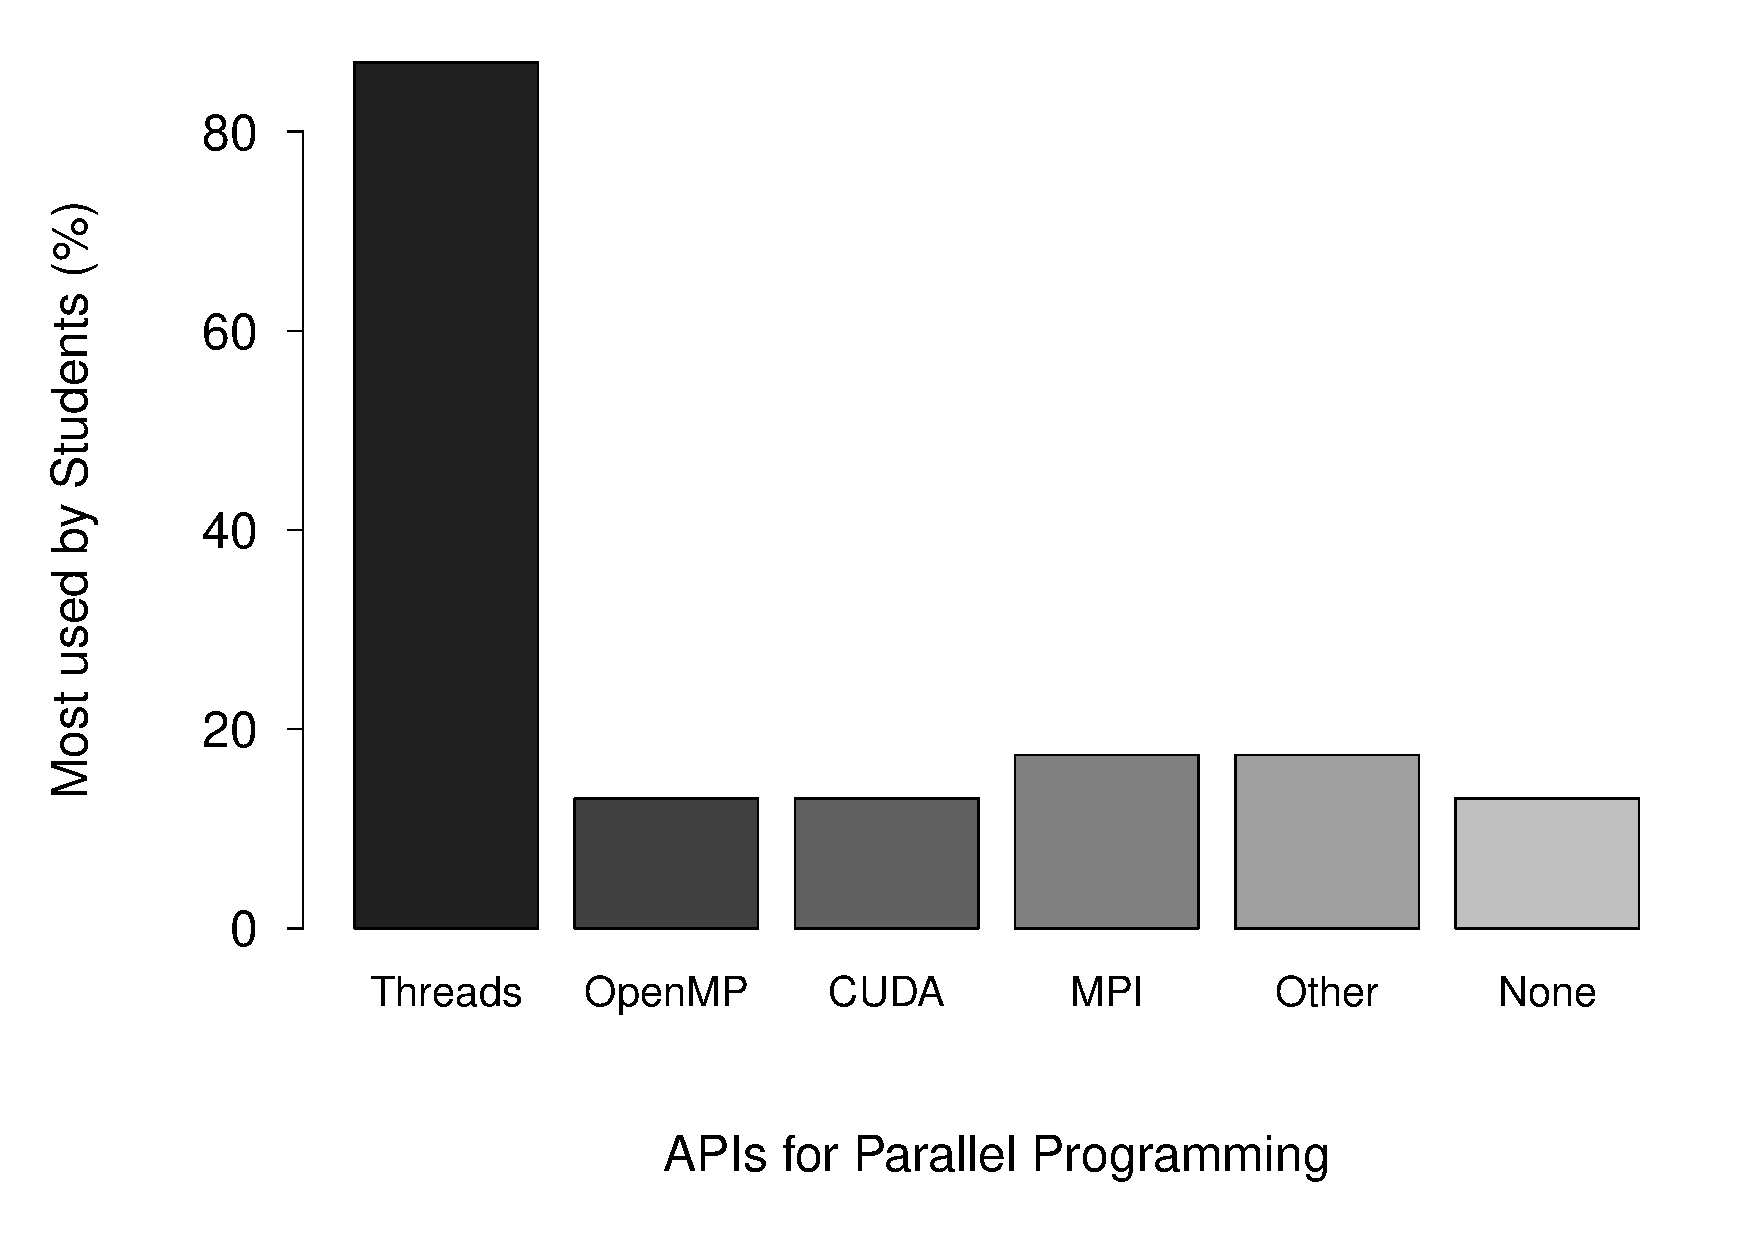
\includegraphics[width=0.95\columnwidth,height=0.65\columnwidth]{figures/experiencePP.eps}
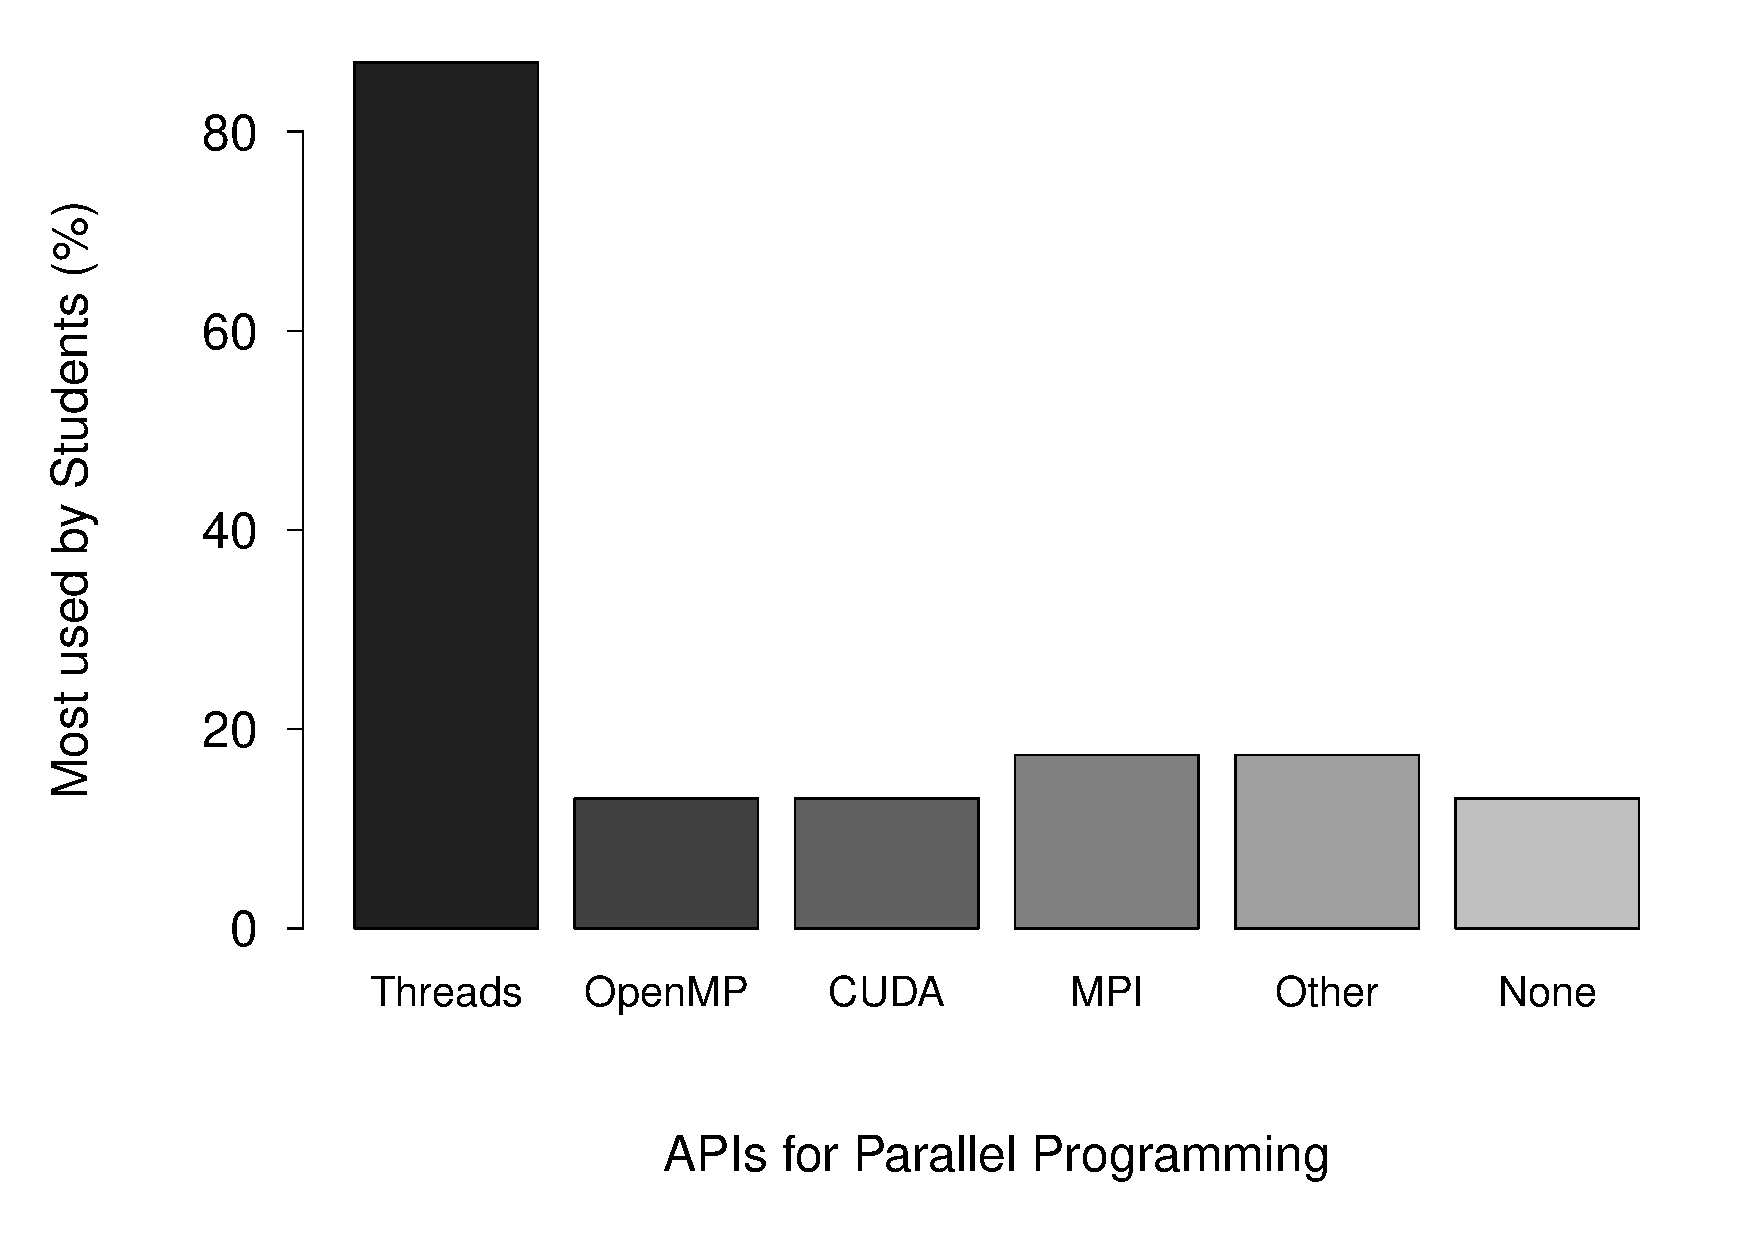
\includegraphics[width=1.0\columnwidth,height=0.70\columnwidth, trim={0 1.0cm 0 1.5cm},clip]{figures/experiencePP.pdf}
\caption{APIs for Parallel Programming previously used by the students}
\label{fig:students:experience}
\end{figure}

The other question was about the programming languages known by the students. The objective of this information was to measure how easy it is to learn \texttt{OpenMP} when you know the basic concepts and what is the influence that the knowledge of other languages can have on the process. Figure~\ref{fig:LangMoreUsed} presents the distribution of programming languages known for the students involved in the experiment.

\begin{figure}[htpb]
\centering
% 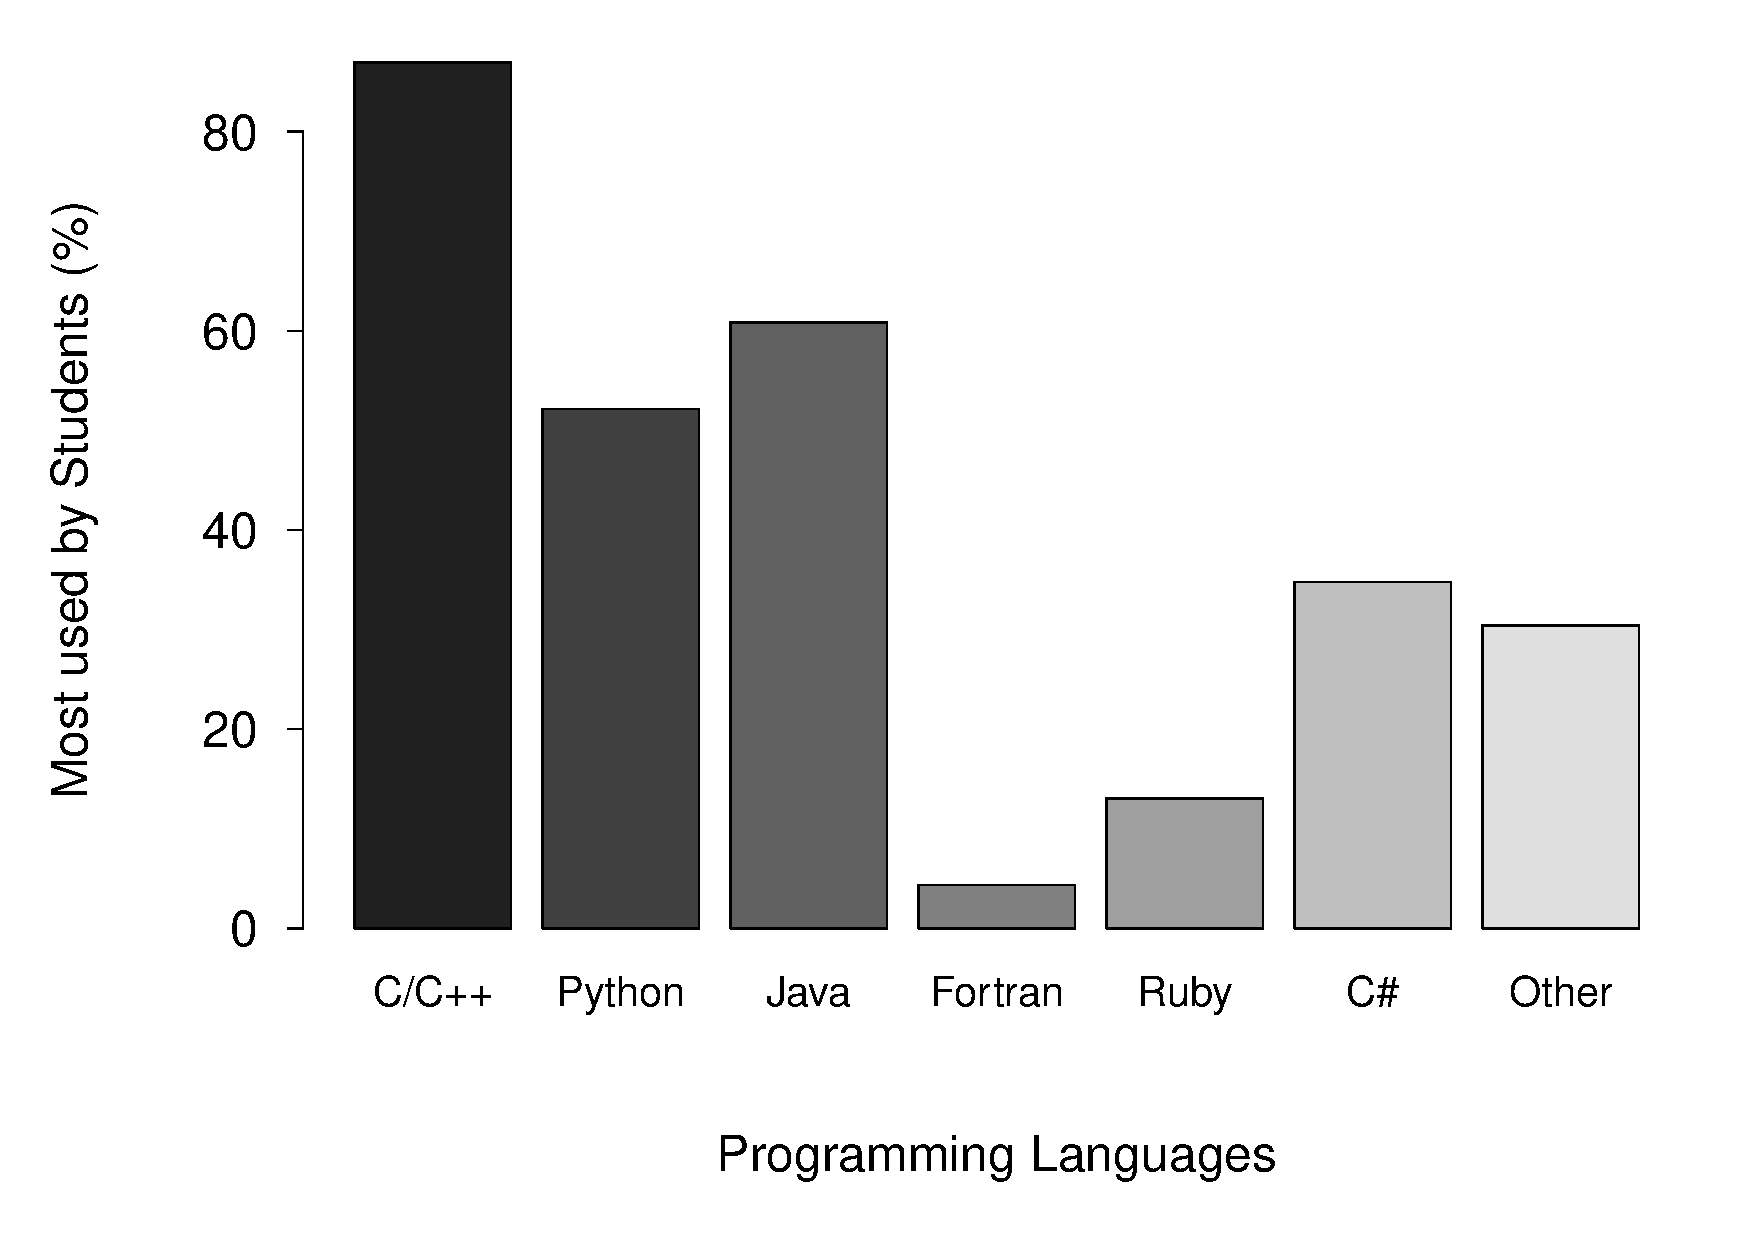
\includegraphics[width=0.95\columnwidth,height=0.65\columnwidth]{figures/experienceLP.eps}
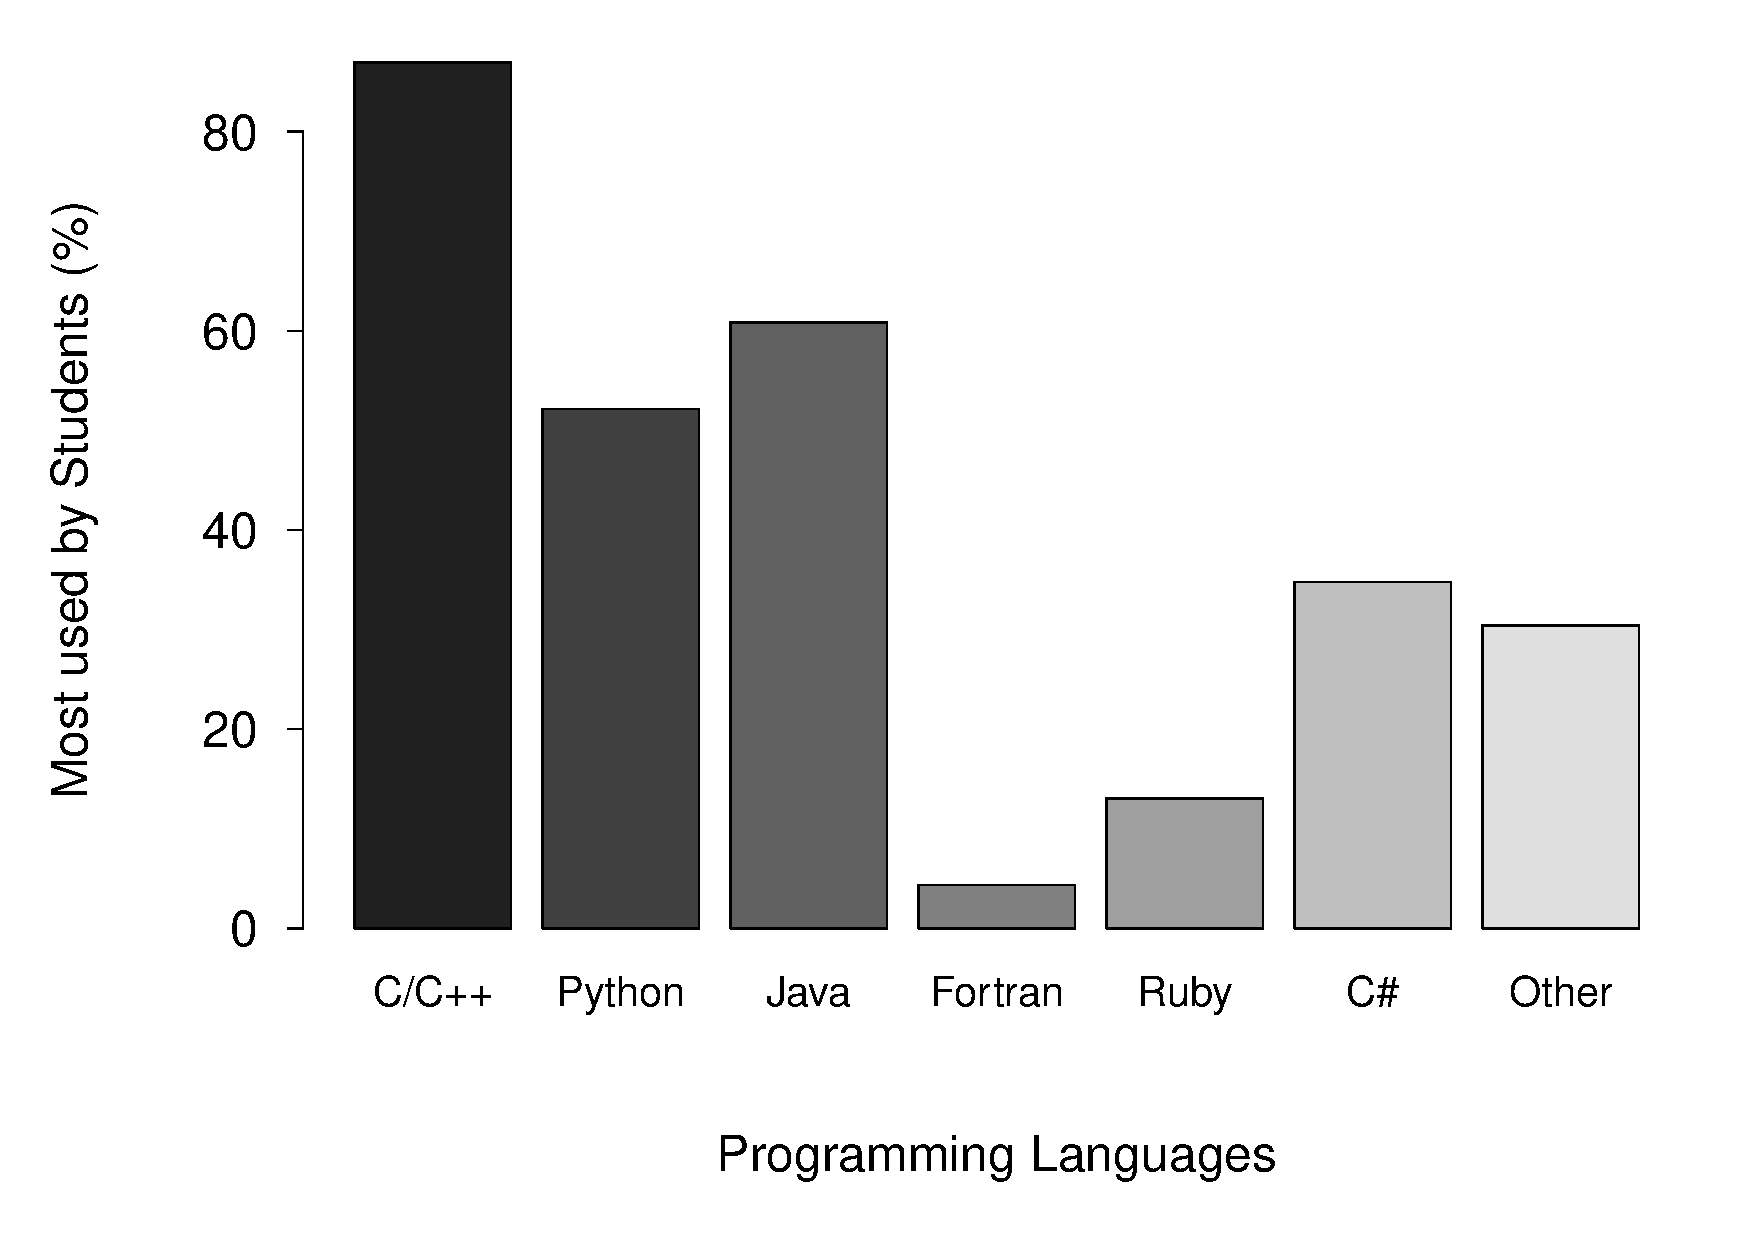
\includegraphics[width=1.0\columnwidth,height=0.70\columnwidth, trim={0 1.0cm 0 1.5cm},clip]{figures/experienceLP.pdf}
\caption{Programming Languages more used by the students}
\label{fig:LangMoreUsed}
\end{figure}